\documentclass{article}

\usepackage{graphicx}
\usepackage{tikz}
\usepackage{tikzsymbols}
\usetikzlibrary{calc,patterns,shapes.geometric}
\pagestyle{empty}
\usepackage[margin=0pt]{geometry}
\geometry{papersize={14in,12in}}

\def\centerarc[#1](#2)(#3:#4:#5){\draw[#1] ($(#2)+({#5*cos(#3)},{#5*sin(#3)})$) arc (#3:#4:#5);}

\begin{document}
	\begin{figure}
		\centering
		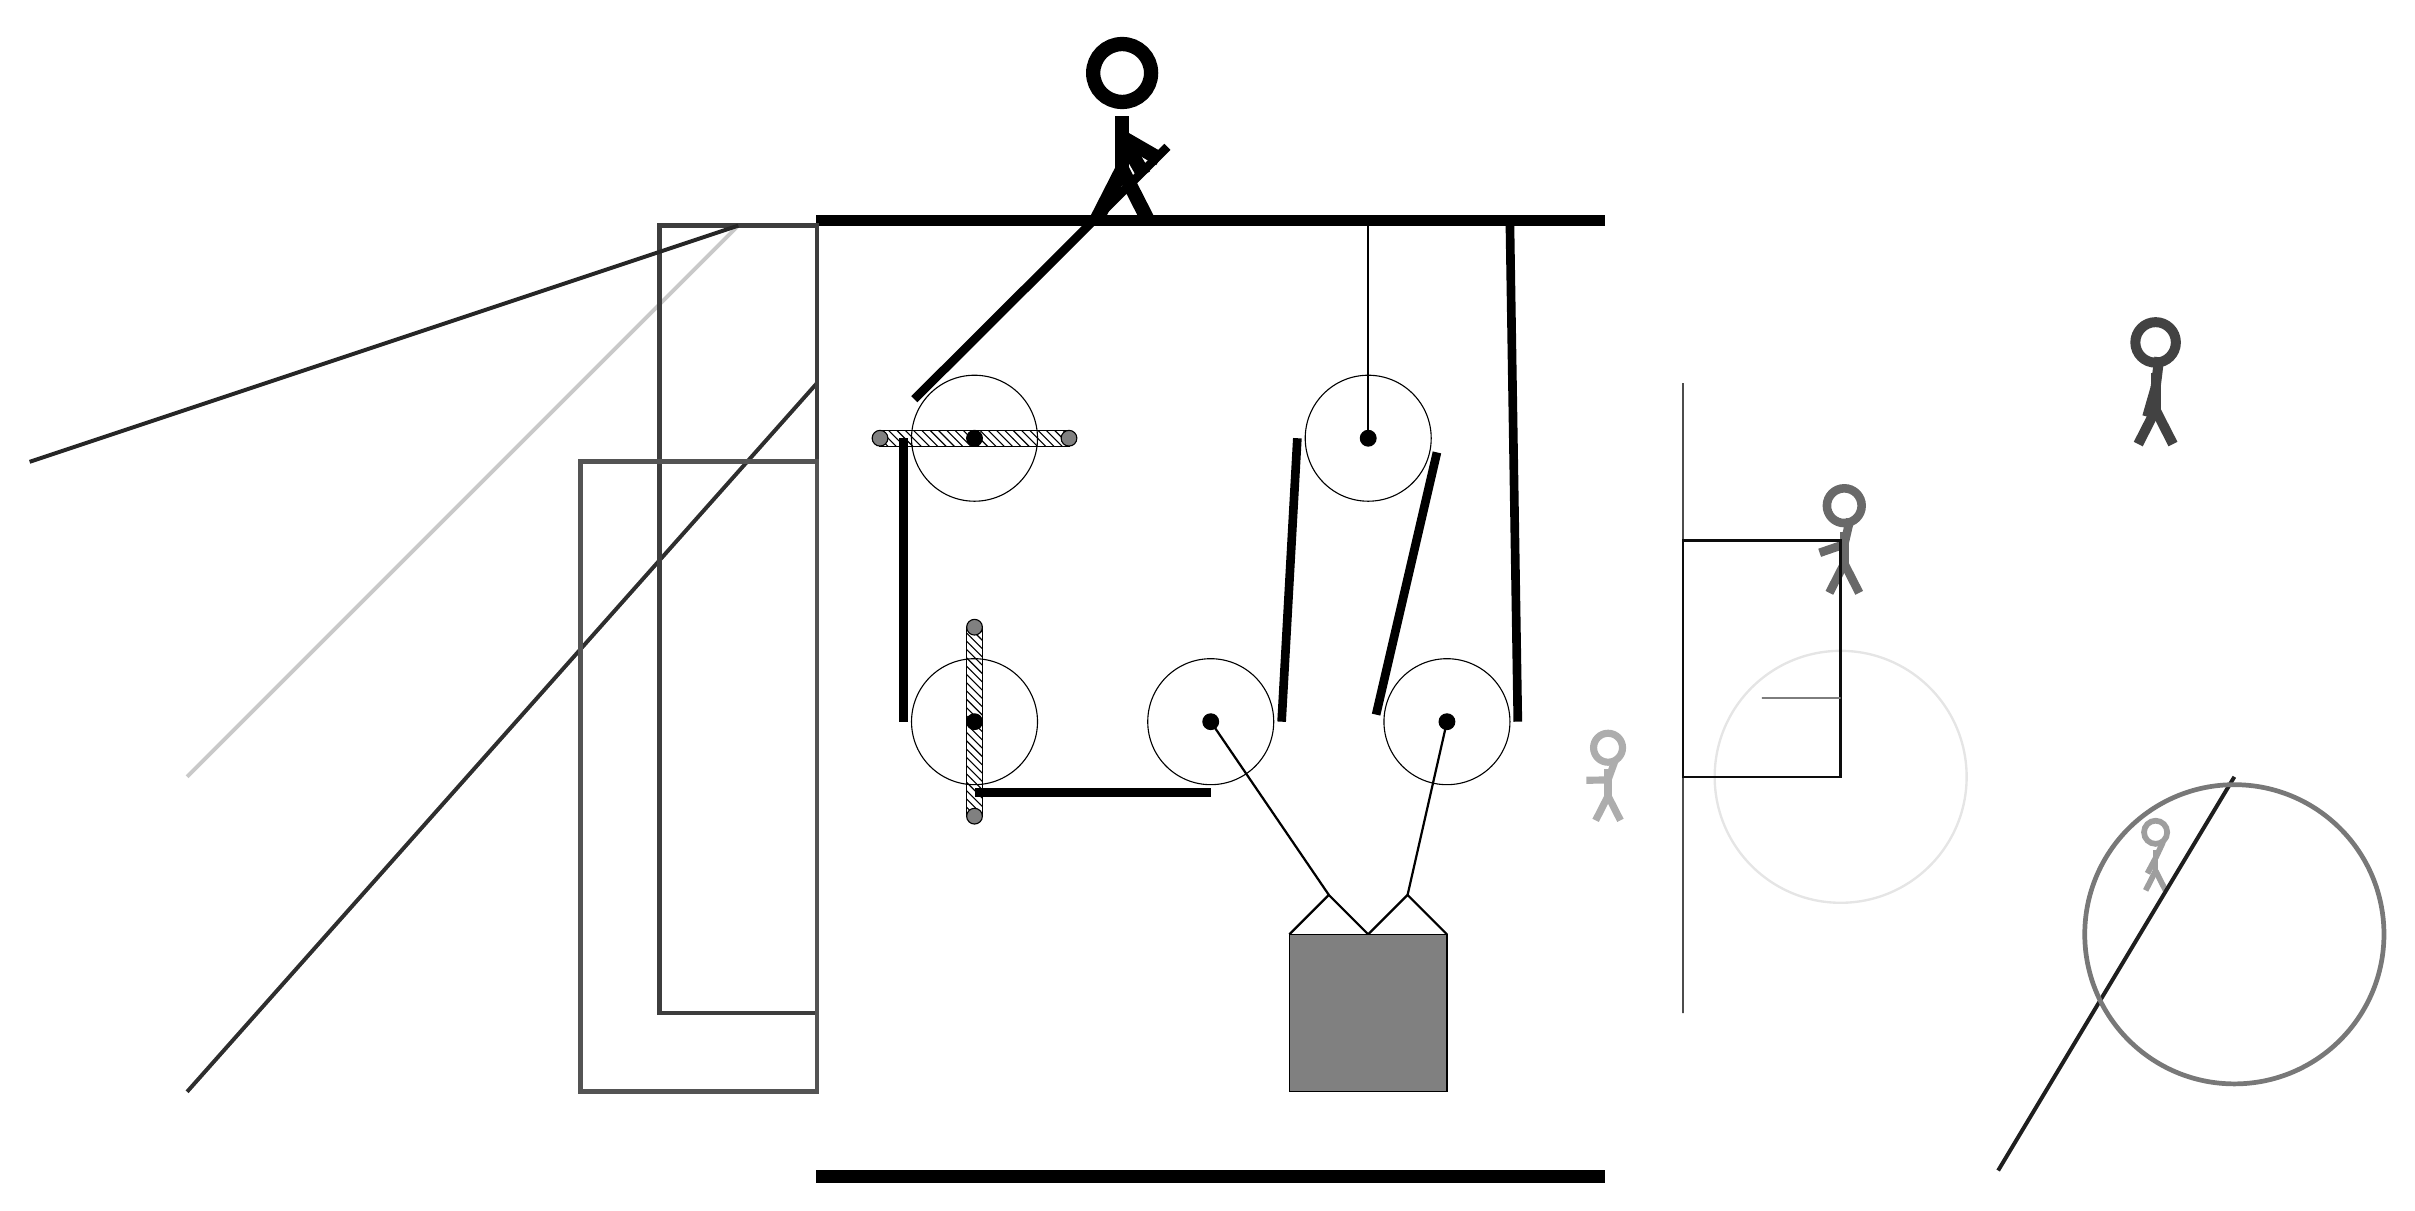
\begin{tikzpicture}
			%%%%% START %%%%%
			
			\draw[fill=black] (-4, 9) rectangle (6, 9.125);
			
			\draw (1, 2.7) circle (0.8);
			\draw[fill=black] (1, 2.7) circle (0.1);
			
			\draw (3, 6.3) circle (0.8);
			\draw[fill=black] (3, 6.3) circle (0.1);
			\draw[thick] (3, 6.3) -- (3, 9);
			
			\draw (4, 2.7) circle (0.8);
			\draw[fill=black] (4, 2.7) circle (0.1);
			
			\draw[thick] (4, 2.7) -- (3.5, 0.5);
			\draw[thick] (1, 2.7) -- (2.5, 0.5);
			\draw[thick]  (2, 0) -- (2.5, 0.5) -- (3, 0);
			\draw[thick]  (3, 0) -- (3.5, 0.5) -- (4, 0);
			\draw[fill=black!50] (2, 0) rectangle (4, -2);
			
			\draw[line width=0.5mm, color=black!82](-4, 7) -- (-12, -2);
			
			\draw [line width=0.3mm, color=black!10](9, 2) circle (1.6);
			\node[line width=0.7mm, color=black!38] at (13, 1) {\Strichmaxerl[4][62][65]};
			\node[line width=0.3mm, color=black!59] at (9, 5) {\Strichmaxerl[6][19][77]};
			\draw [line width=0.2mm, color=black!56](-9, 8) circle (0.0);
			\draw[line width=0.2mm, color=black!70] (7, 7) rectangle (7, -1);
			\draw[line width=0.5mm, color=black!88](11, -3) -- (14, 2);
			
			\draw[line width=0.3mm, color=black!95] (7, 5) rectangle (9, 2);
			\draw[line width=0.5mm, color=black!21](-5, 9) -- (-12, 2);
			
			\draw [line width=0.6mm, color=black!53](14, 0) circle (1.9);
			\draw[line width=0.6mm, color=black!76] (-4, 9) rectangle (-6, -1);
			
			\draw[line width=0.3mm, color=black!51] (8, 3) rectangle (9, 3);
			\node[line width=0.3mm, color=black!74] at (13, 7) {\Strichmaxerl[7][74][83]};
			
			\draw[line width=0.6mm, color=black!67] (-4, -2) rectangle (-7, 6);
			\draw[line width=0.5mm, color=black!85](-5, 9) -- (-14, 6);
			\node[line width=0.3mm, color=black!32] at (6, 2) {\Strichmaxerl[5][1][70]};
			
			
			\draw (-2, 2.7) circle (0.8);
			\draw[fill=black] (-2, 2.7) circle (0.1);
			\draw[pattern=north west lines, pattern color=black] (-2.1, 3.9) rectangle (-1.9, 1.5);
			\draw[fill=black!50] (-2, 3.9) circle (0.1);
			\draw[fill=black!50] (-2, 1.5) circle (0.1);
			
			\draw (-2, 6.3) circle (0.8);
			\draw[fill=black] (-2, 6.3) circle (0.1);
			\draw[pattern=north west lines, pattern color=black] (-3.2, 6.4) rectangle (-0.8, 6.2);
			\draw[fill=black!50] (-3.2, 6.3) circle (0.1);
			\draw[fill=black!50] (-0.8, 6.3) circle (0.1);
			
			\draw[line width=1.1mm] (0.45, 10) -- (-2.765, 6.795);
			\centerarc[line width=1.1mm](-2, 6.3)(135:180:0.9);
			\draw[line width=1.1mm] (-2.9, 6.3) -- (-2.9, 2.7);
			\centerarc[line width=1.1mm](-2, 2.7)(180:270:0.9);
			\draw[line width=1.1mm](-2, 1.8) -- (1, 1.8);
			\centerarc[line width=1.1mm](1, 2.7)(270:360:0.9);
			\draw[line width=1.1mm] (1.9, 2.7) -- (2.1, 6.3);
			\centerarc[line width=1.1mm](3, 6.3)(-20:180:0.9);
			\draw[line width=1.1mm](3.873, 6.12) -- (3.1, 2.79);
			\centerarc[line width=1.1mm](4, 2.7)(160:360:0.9);
			\draw[line width=1.1mm](4.9, 2.7) -- (4.8, 9);
			
			\node at (-0.07, 10.2) {\Strichmaxerl[10][120][-30]};
			
			\draw[fill=black] (-4, -3) rectangle (6, -3.15);
			
			%%%%% END %%%%%
		\end{tikzpicture}
	\end{figure}	
\end{document}